% Presenting ReaxFF
    \subsection{Présentation de \reaxff{}} \label{sec:reaxff}

\begin{figure}[h!]
    \centering
    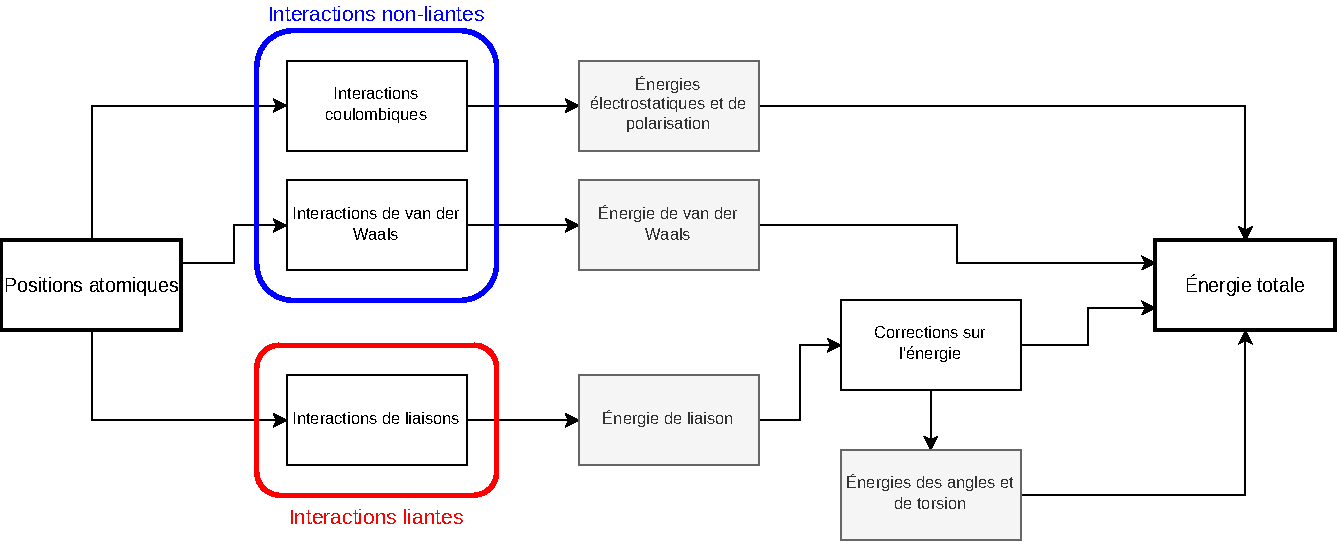
\includegraphics[width=\linewidth]{H2O-ReaxFF-interactions.pdf}
    \caption{Interactions et énergies au sein de \reaxff{} (tiré de \cite{russo_atomistic-scale_2011})}
    \label{fig:interactions_energies_reaxff}
\end{figure}

\reaxff{}\cite{russo_atomistic-scale_2011}\cite{senftle_reaxff_2016} est un potentiel qui utilise les ordres de liaison pour modéliser les réactions chimiques (\autoref{fig:interactions_energies_reaxff}), prend en compte les interaction non-liantes, et effectue  une équilibration de charges.\\
Il a été conçu de façon à obtenir des résultats dont la précision se rapproche des méthodes quantiques, en mettant en jeu autant d'atomes que les méthodes classiques.\\
Enfin, ce potentiel a été comparé à un modèle existant de la molécule d'eau à la \autoref{sec:h2o}.

\textbf{Ordres de liaisons}\\
L'ordre d'une liaison entre un atome $i$ et un atome $j$ est donné par :
\begin{equation}
    BO_{ij}' = \exp \left[p_{bo, 1} \left(\frac{r_{ij}}{r_o}\right)^{p_{bo,2}}\right] + \exp \left[p_{bo,3} \left(\frac{r_{ij}^\pi}{r_o}\right)^{p_{bo,4}}\right] + \exp \left[p_{bo,5} \left(\frac{r_{ij}^{\pi\pi}}{r_o}\right)^{p_{bo,6}}\right]
    \label{eq:ordres_liaisons_reaxff}
\end{equation}
où paramètres $p_{bo,1}, \dots, p_{bo,6}, r_o$ sont des pamramètres issus de calculs \textit{ab initio}, et dépendent de la nature des atomes mis en jeu, et du type de liaison considéré. Les ordres de liaisons sont ensuite corrigés pour être intégrés aux calculs des énergie de liaisons, d'angles et de torsions.

\textbf{Interactions non-liantes}\\
\reaxff{} inclue également les interactions de \vdw{} et \coulomb{} pour \emph{toutes} les paires d'atomes. Les interactions de \vdw{} se basent sur un potentiel de Morse, et ces deux types d'interactions sont protégées par un paramètre $\gamma$ pour éviter de trop grandes attractions et répulsions (\autoref{fig:reaxff_vdw_coulomb}).

\begin{figure}[h!]
    \centering
    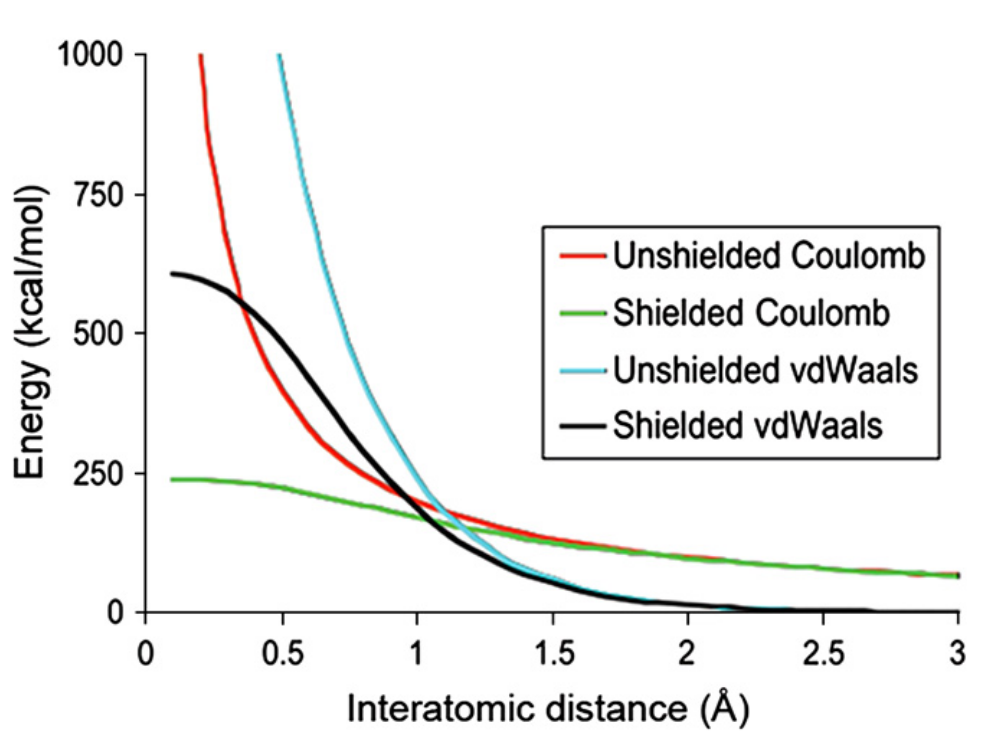
\includegraphics[height = 5 cm]{reaxff_vdw_coulomb.png}
    \caption{Allures des énergies des interactions de \vdw{} et \coulomb{} protégées {\tiny (tiré de \cite{russo_atomistic-scale_2011})}}
    \label{fig:reaxff_vdw_coulomb}
\end{figure}

\textbf{Équilibration des charges}\\
\reaxff{} utilise une méthode d'équilibration des charges, effectuée à chaque pas de temps, basée sur l'\emph{Electron Equilibration Method} (abrégé \eem{})\cite{mortier_electronegativity-equalization_2002} et la méthode \qeq{}\cite{rappe_charge_1991} :
\begin{equation}
    \boxed%
    {
    \frac{\partial E}{\partial q_i} = \chi_i + 2 q_i H_i + C \sum_{j \neq i} \frac{q_j}{\left(r_{ij}^3 + (1 / \gamma_{ij})^3\right)^{1/3}}
    }
    \ \text{ et } \ 
    \boxed%
    {
        \sum_{i = 1}^{N_{atomes}} q_i = 0
    }
\end{equation}
où $q_i$ est la charge d'un atome $i$, $\chi_i$ son électronégativité, $H_i$ sa dureté, $r_{ij}$ est la distance entre un atome $i$ et un atome $j$ et $\gamma_{ij}$ est le paramètre de protection pour la paire $ij$.


% Presenting EChemDID
    \subsection{Présentation d'\echemdid{}} \label{sec:echemdid}

\begin{figure}[h!]
    \centering
    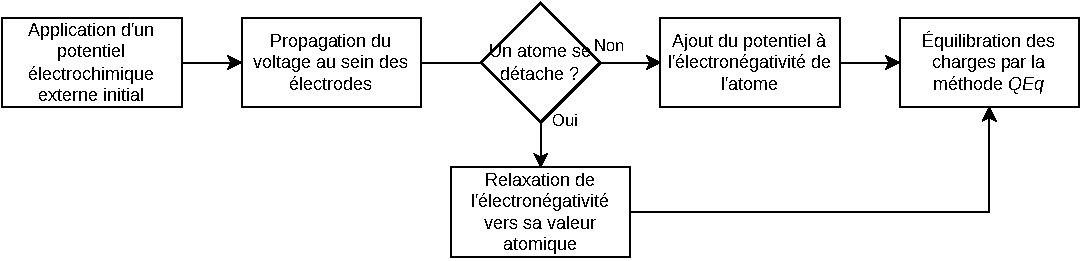
\includegraphics[height = 3 cm]{echemdid_methode.pdf}
    \caption{Fonctionnement d'\echemdid{}}
    \label{fig:echemdid_fonctionnement}
\end{figure}

\textbf{Application d'un potentiel électrochimique externe}\\
Pour fonctionner, \echemdid{} assigne à chaque atome un potentiel électrochimique local $\Phi_i (t)$ et applique initialement un potentiel électrochimique externe à un groupe prédéfini d'atomes.

\textbf{Propagation du voltage au sein des électrodes}\\
Le but d'\echemdid{} étant de représenter les réactions électrochimiques, la progpagation du voltage au sein des électrodes se fait simplement selon la relation :
\begin{equation}
    \dot{\Phi} = k \Delta \Phi
    \label{eq:echemdid_propagation}
\end{equation}
où $k$ est un coefficient de diffusion, et $\Delta$ est l'opérateur Laplacien. Pour résoudre cette équation, \echemdid{} suppose que chaque atome se situe dans un réseau de référence (ou grille).

Pour résoudre cette équation, plusieurs points sont à prendre en compte :
\begin{itemize}
    \item si une différence de potentiel est appliquée entre deux électrodes, le voltage devra s'équilibrer en une durée dépendant du coefficient $k$
    \item si un atome se détache d'une électrode, son électronégativité devra progressivement revenir à sa valeur atomique notée $\chi_i^0$
\end{itemize}

La solution numérique de cette équation peut alors être exprimée :
\begin{equation}
    \boxed%
    {
        \dot{\Phi}_i (t) = \sum_{j \neq i} \frac{\Phi_i (t) - \Phi_j (t)}{{R_{ij}}^2}w(R_{ij}) + \eta F(W_i) \Phi_i
    }
    \label{eq:echemdid_solution_numerique}
\end{equation}
où $R_{ij} = | \vec{r}_i - \vec{r}_j |$, $\vec{r}_i$ est la position de l'atome dans la grille, $w(R)$ est une fonction de poids, $\eta$ est un coefficient de relaxation, $F(W)$ est une fonction d'activation de la relaxation, et $W_i$ est la coordinance métallique totale de l'atome $i$.

Le premier terme à droite de cette équation résout l'équation de la diffusion du voltage aux seins des électrodes, et la fonction de poids a pour expression :
\begin{equation*}
    w(R) = \left\{
        \begin{aligned}
            &\mathcal{N} \left[ 1 - \left(\frac{R}{R_c}\right)^2 \right]^2 &\text{si } R < R_c\\
            &0 &\text{sinon}
        \end{aligned}
    \right.
\end{equation*}
où $R_c$ est la distance maximale à partir de laquelle deux atomes ne sont plus considérés comme faisant partie du même amas métallique, $\mathcal{N} = \frac{2 d N_{atomes}}{\sum_{i} W_i}$ est un coefficient de normalisation, $d$ est le nombre de dimensions du problème, et $W_i = \sum_{j \neq i} w(R_{ij})$ est la coordinance métallique totale de l'atome $i$ sur la grille.

Quant au second terme à droite, il permet d'activer la relaxation de l'électronégativité, et la fonction d'activation a pour expression :
\begin{equation*}
    F(W) = \left\{
        \begin{aligned}
            &\left[ 1 - \left( \frac{W}{W_0}\right)^2\right]^2 &\text{si } W < W_0\\
            &0 &\text{sinon}
        \end{aligned}
    \right.
\end{equation*}
où $W_0$ est la coordinance métallique minimale en dessous de laquelle l'électronégativité doit tendre vers sa valeur atomique, en général on prend $W_0 = w(\num{0.99}R_c)$.

La \autoref{fig:echemdid_allures_w_f} montre l'allure des fonctions $w$ et $F$ pour un réseau cristallin de graphite de \num{540} atomes, en supposant que pour tous les atomes on a $W_i = \num{3}$ et en prenant $R_c = \qty{4}{\angstrom}$.

\begin{figure}[h!]
    \centering
    \begin{subfigure}{\textwidth}
        \centering
        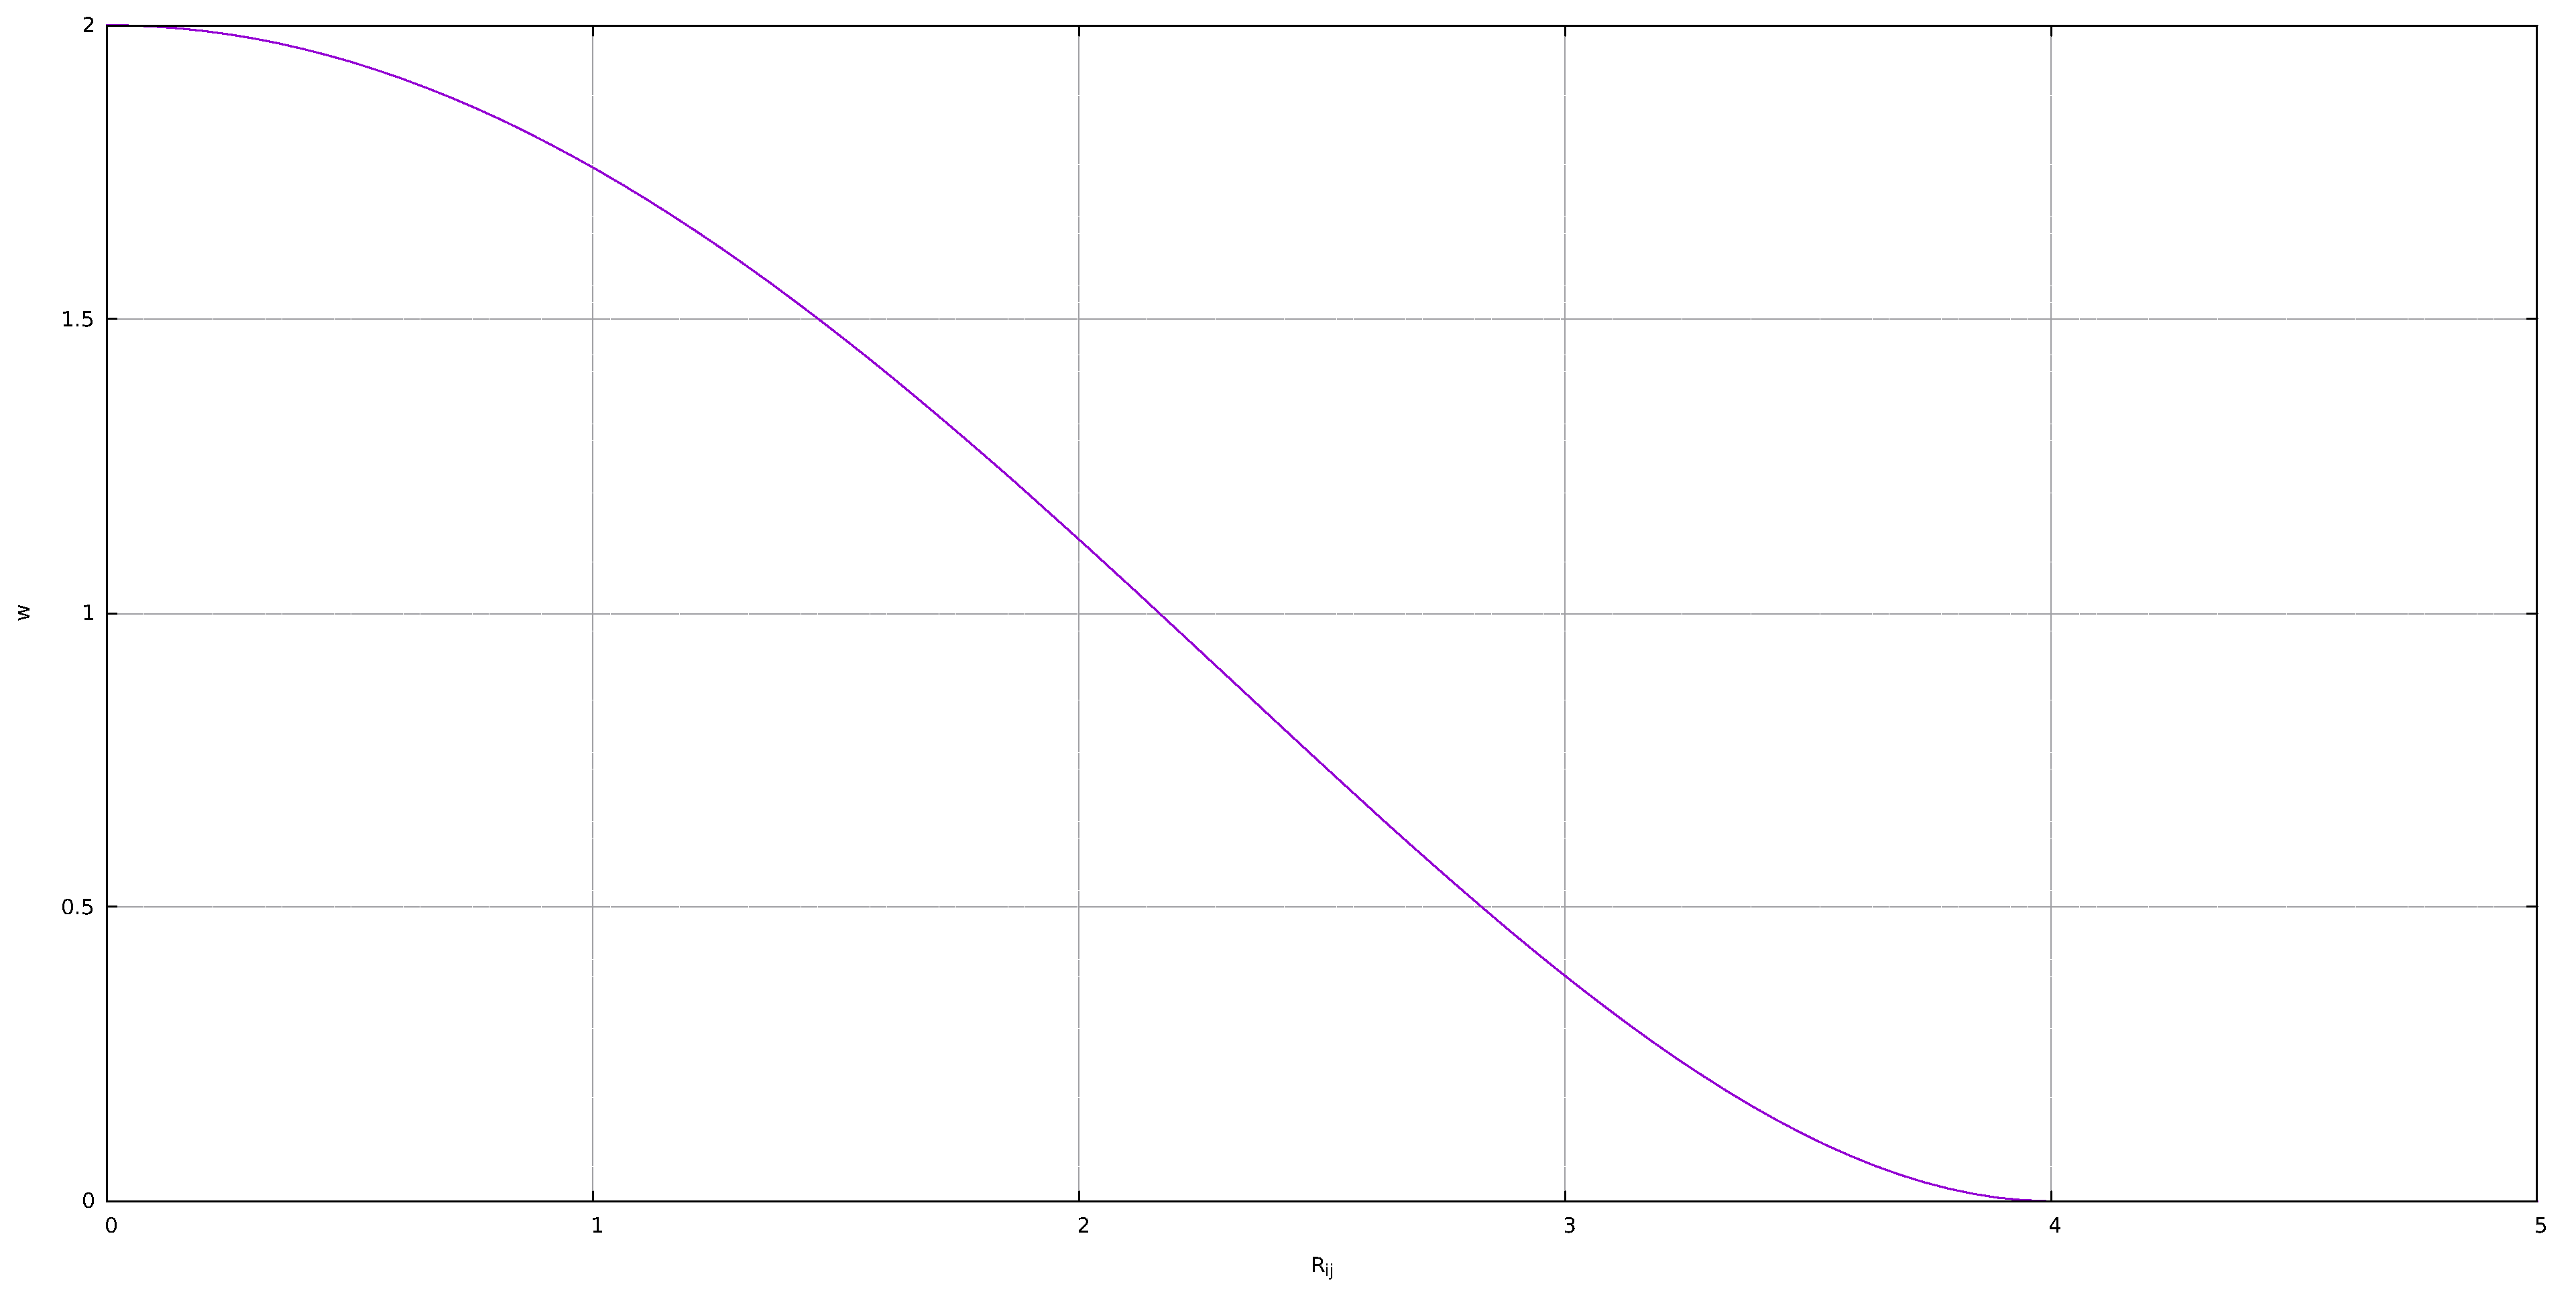
\includegraphics[height = 6 cm]{echemdid_allure_w.pdf}
        \caption{$w(R)$}
    \end{subfigure}
    \begin{subfigure}{\textwidth}
        \centering
        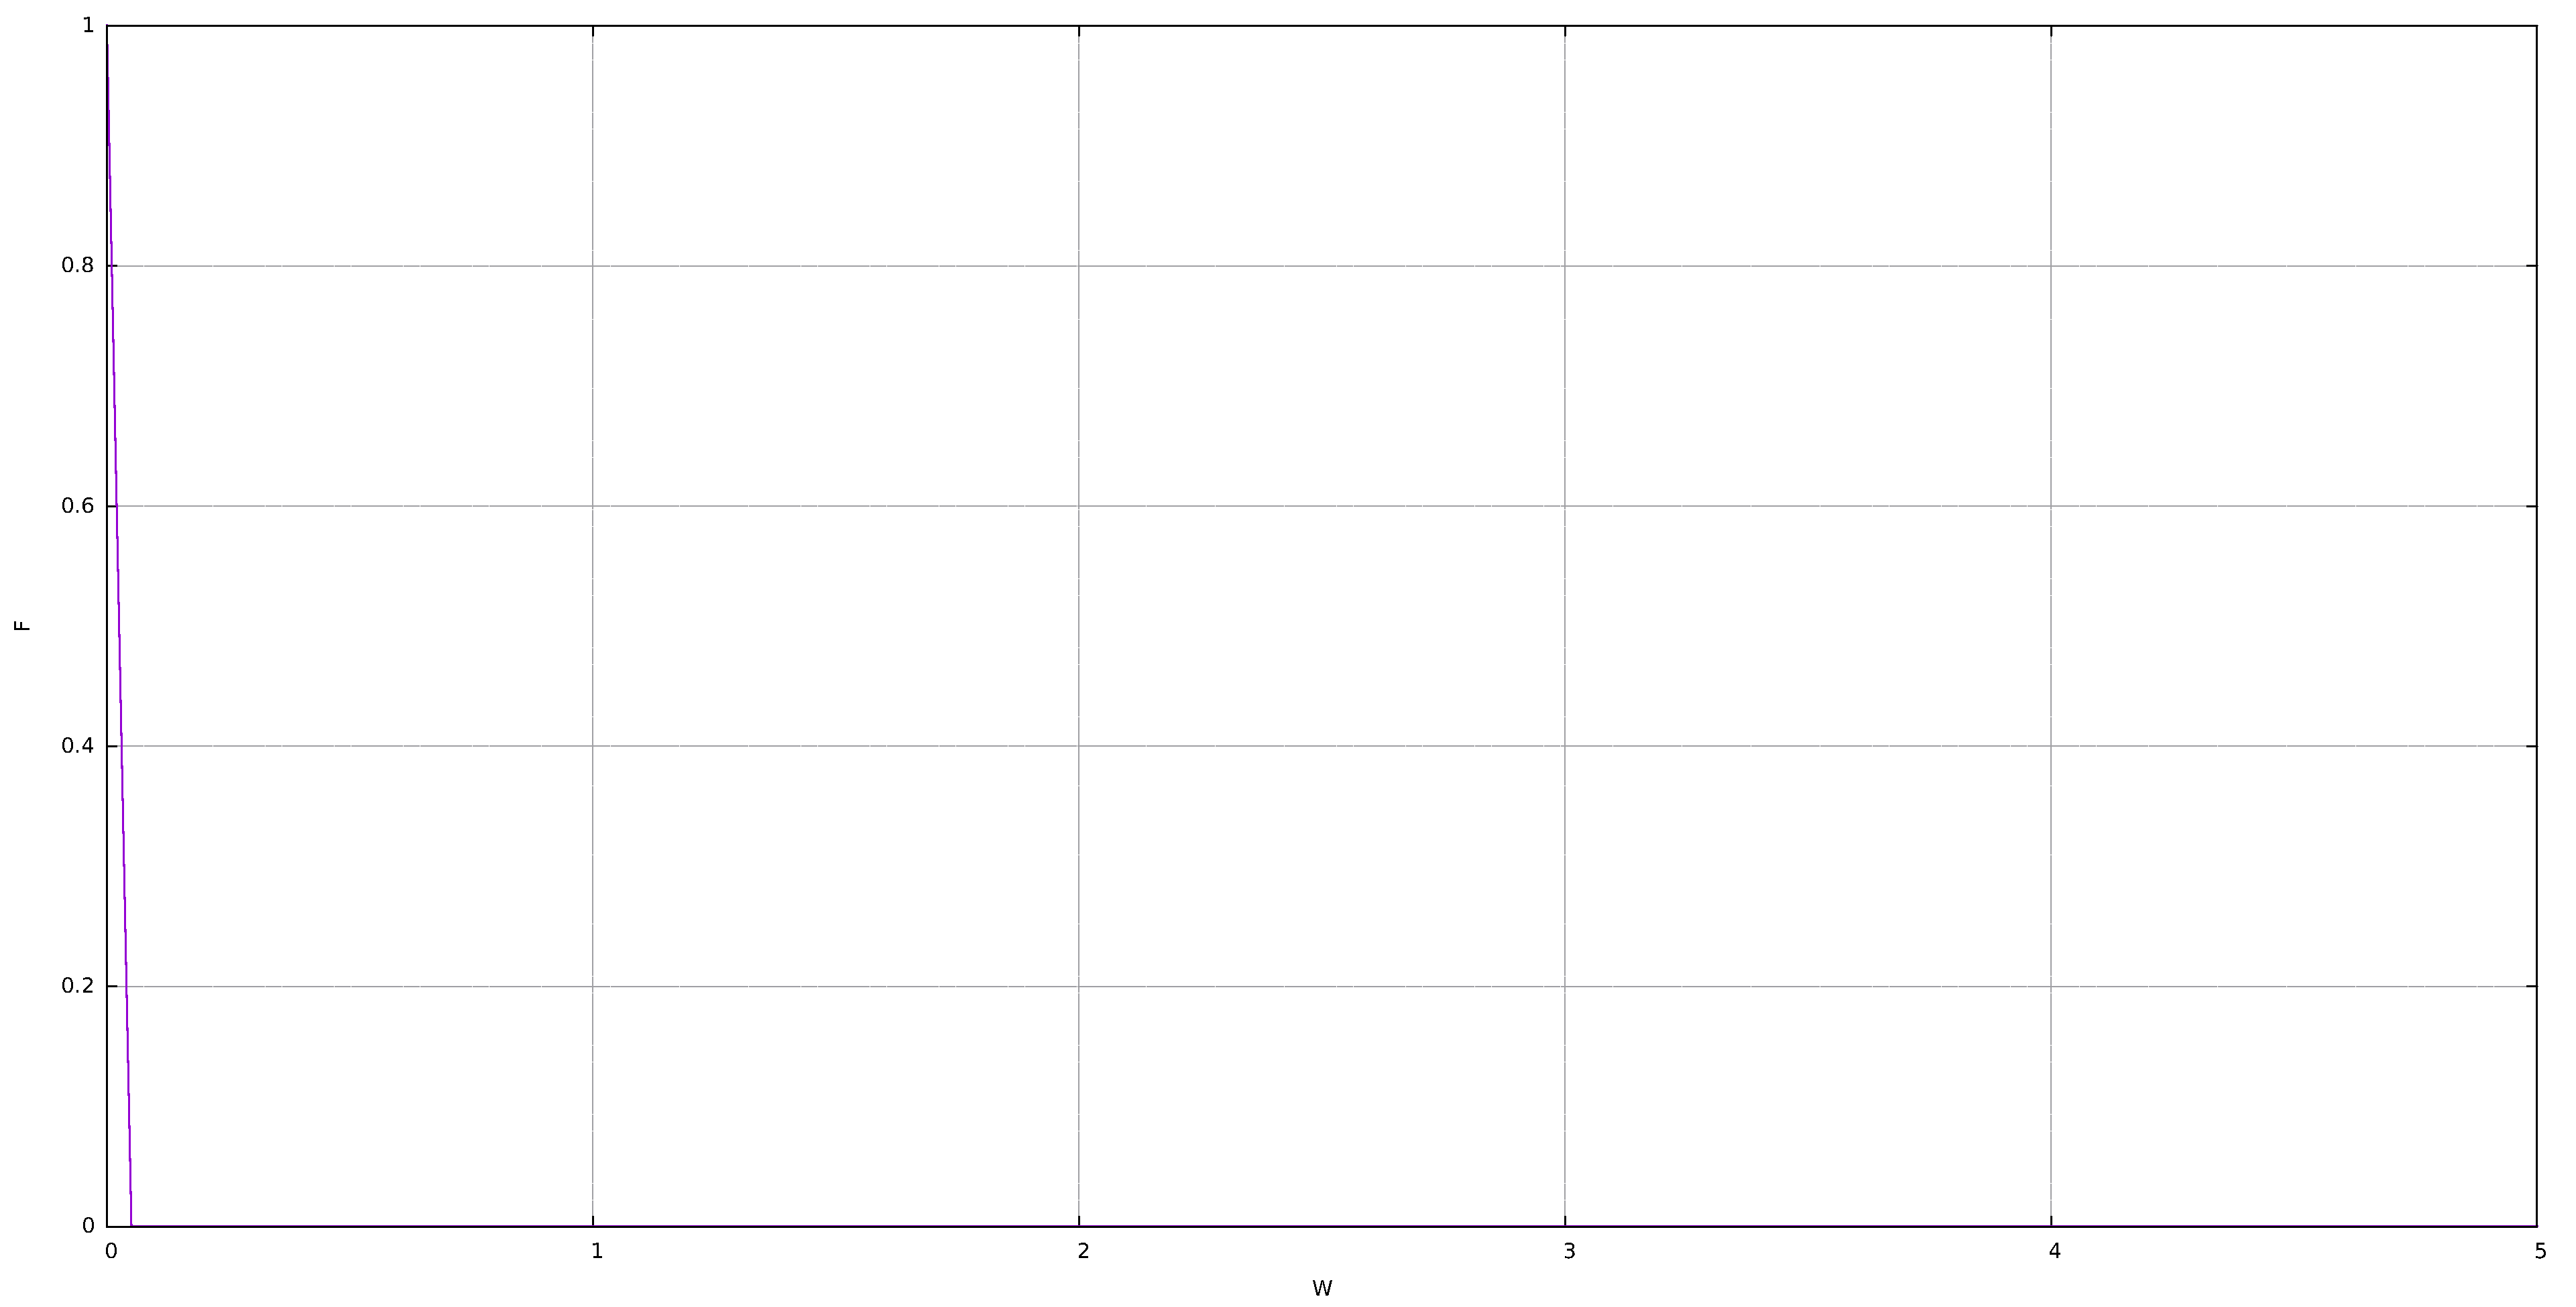
\includegraphics[height = 6 cm]{echemdid_allure_f.pdf}
        \caption{$F(W)$}
    \end{subfigure}
    \begin{subfigure}{\textwidth}
        \centering
        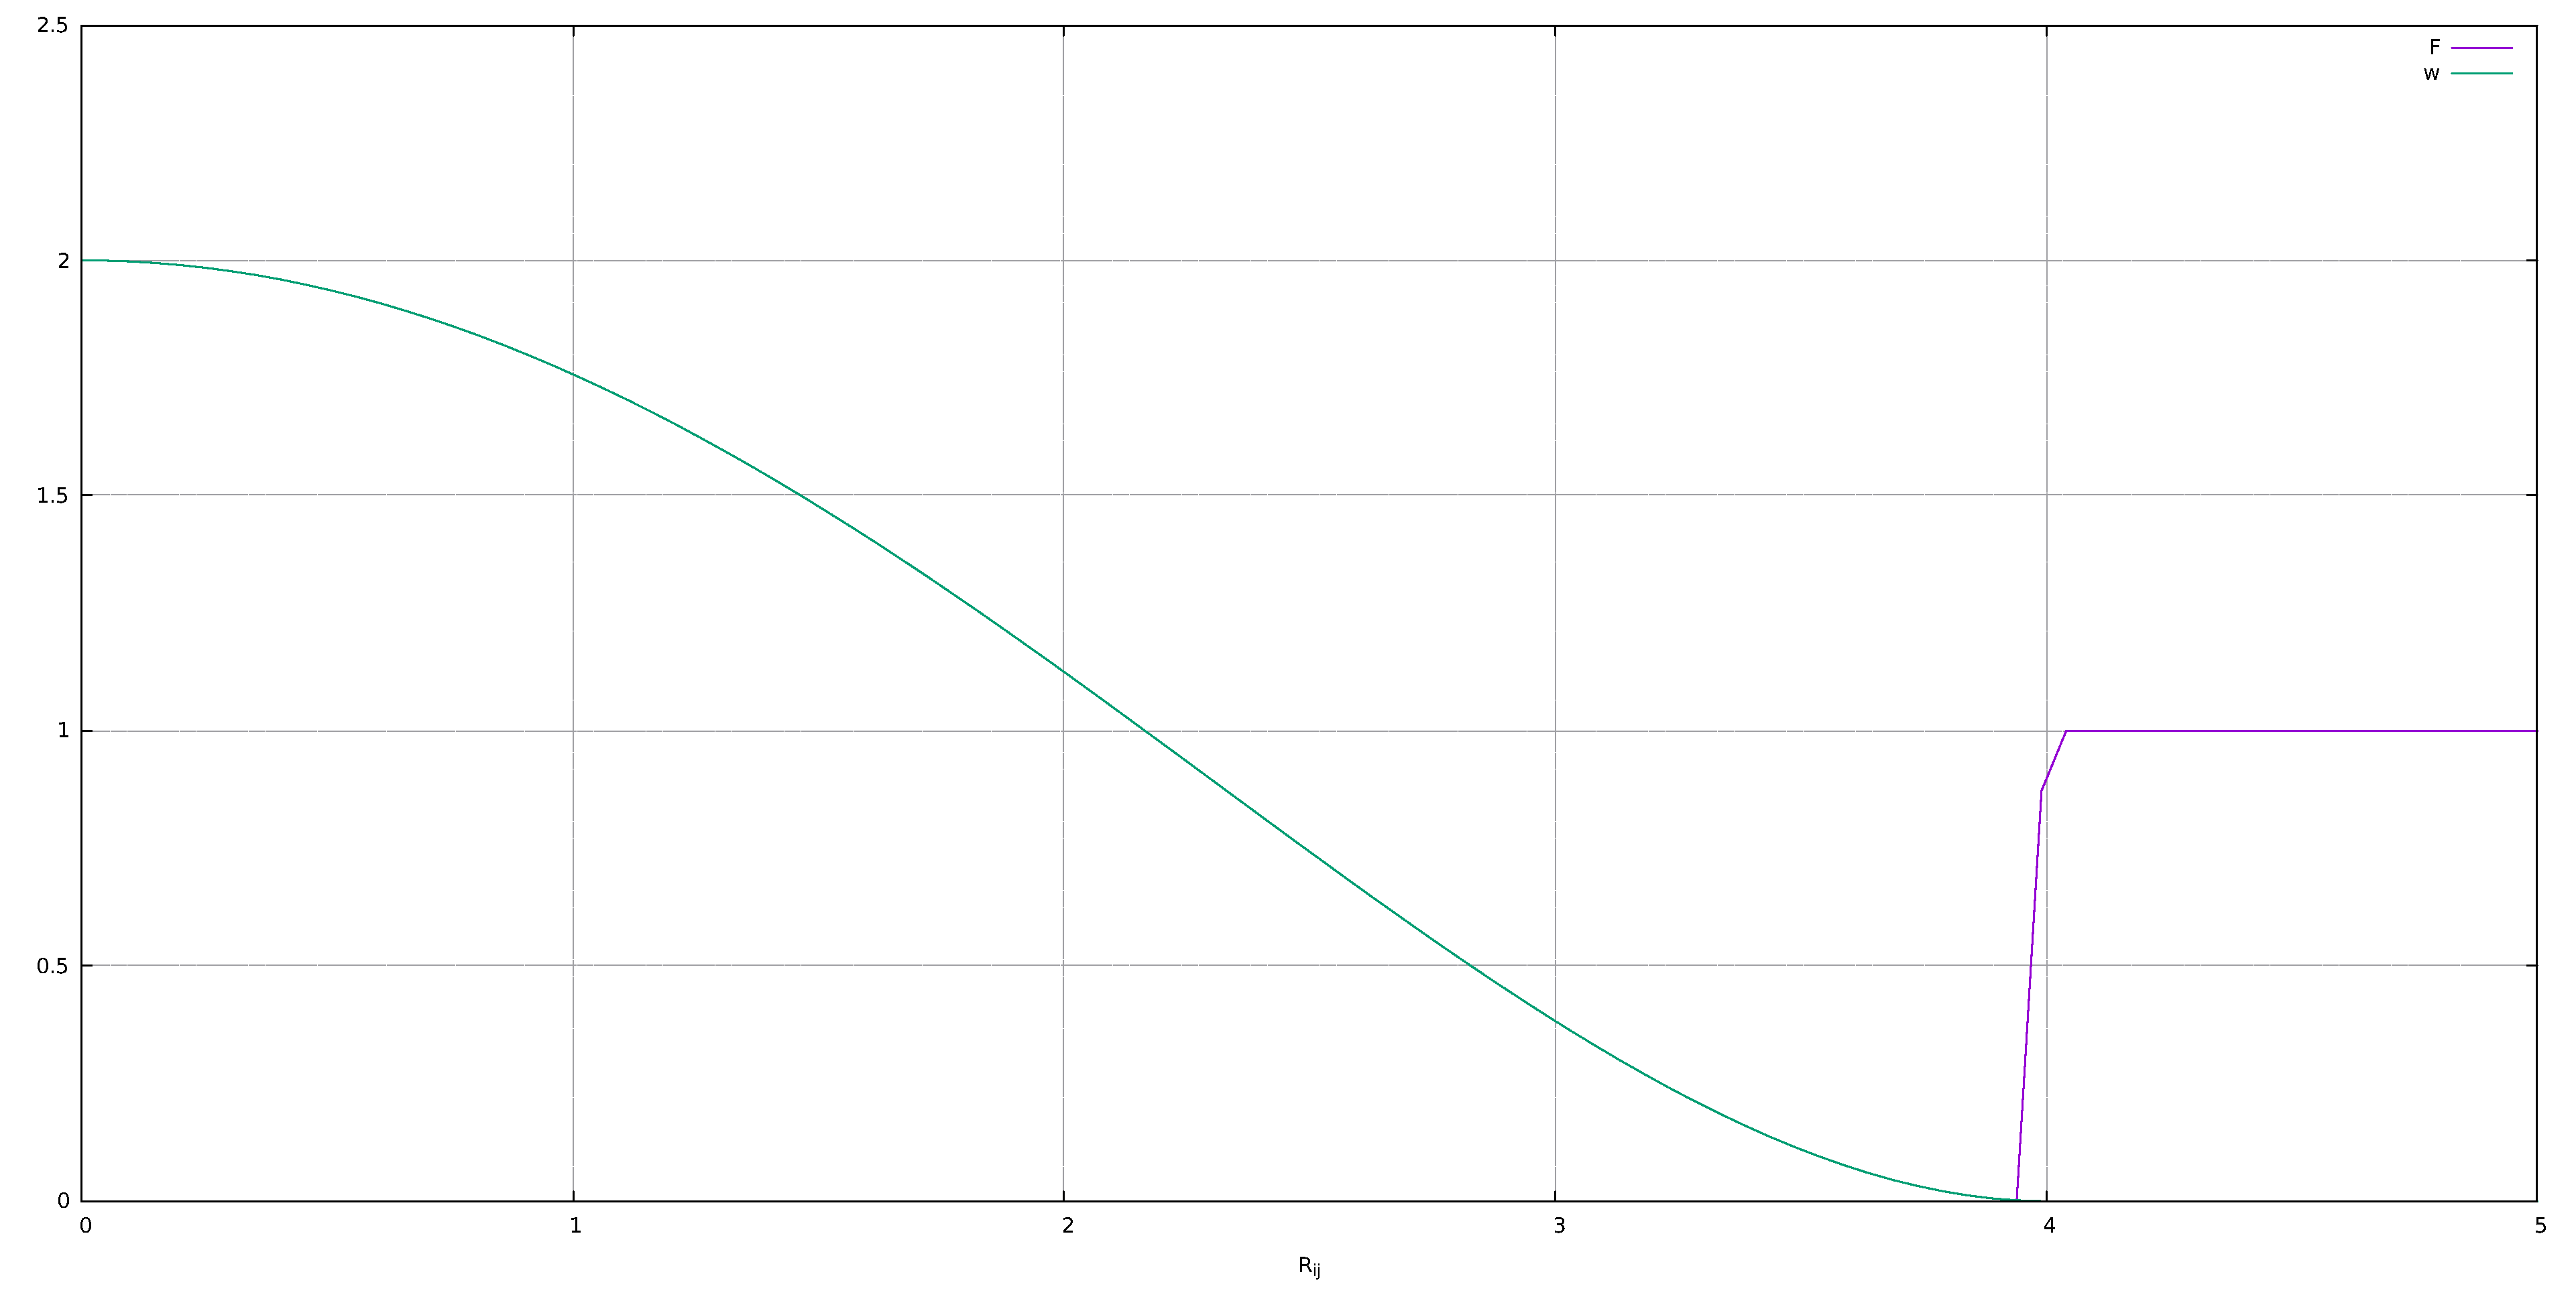
\includegraphics[height = 6 cm]{echemdid_allures_w_f.pdf}
        \caption{$w(R)$ et $F(R) \simeq F(w(R))$}
    \end{subfigure}
    \caption{Allures des fonctions d'\echemdid{}}
    \label{fig:echemdid_allures_w_f}
\end{figure}

\textbf{Ajout du potentiel à l'électronégativité et équilibration des charges}\\
Le potentiel $\Phi_i (t)$ obtenu après avoir calculé la solution (\ref{eq:echemdid_solution_numerique}) et intégré l'\autoref{eq:echemdid_propagation} est ensuite ajouté à l'électronégativité de l'atome $i$ :
\begin{equation*}
    \boxed%
    {
        \chi_i^* (t) = \chi_i^0 + \Phi_i (t)
    }
\end{equation*}
pour effectuer le calcul d'équilibration des charges par la méthode \qeq{}.
